\documentclass[12pt]{article}
\usepackage[english]{babel}
\usepackage[utf8x]{inputenc}
\usepackage{amsmath}
\usepackage{graphicx}
\usepackage[colorinlistoftodos]{todonotes}

\begin{document}
	
	\begin{titlepage}
		
		\newcommand{\HRule}{\rule{\linewidth}{0.5mm}} % Defines a new command for the horizontal lines, change thickness here
		
		\center % Center everything on the page
		
		%----------------------------------------------------------------------------------------
		%	HEADING SECTIONS
		%----------------------------------------------------------------------------------------
		
		\textsc{\LARGE Central Washington University}\\[1.5cm] % Name of your university/college
		\textsc{\Large High Performance Computing}\\[0.5cm] % Major heading such as course name
		\textsc{\large Spring 2019}\\[0.5cm] % Minor heading such as course title
		
		%----------------------------------------------------------------------------------------
		%	TITLE SECTION
		%----------------------------------------------------------------------------------------
		
		\HRule \\[0.4cm]
		{ \huge \bfseries Project 1 Report}\\[0.4cm] % Title of your document
		\HRule \\[1.5cm]
		
		%----------------------------------------------------------------------------------------
		%	AUTHOR SECTION
		%----------------------------------------------------------------------------------------
		
		\begin{minipage}{0.4\textwidth}
			\begin{flushleft} \large
				\emph{Author:}\\
				Hermann \textsc{Yepdjio} % Your name
			\end{flushleft}
		\end{minipage}
		~
		\begin{minipage}{0.4\textwidth}
			\begin{flushright} \large
				\emph{Supervisor:} \\
				Dr. Szilard \textsc{Vajda} % Supervisor's Name
			\end{flushright}
		\end{minipage}\\[1cm]
		
		% If you don't want a supervisor, uncomment the two lines below and remove the section above
		%\Large \emph{Author:}\\
		%John \textsc{Smith}\\[3cm] % Your name
		
		%----------------------------------------------------------------------------------------
		%	DATE SECTION
		%----------------------------------------------------------------------------------------
		
		{\large \today}\\ % Date, change the \today to a set date if you want to be precise
		
		%----------------------------------------------------------------------------------------
		%	LOGO SECTION
		%----------------------------------------------------------------------------------------
		
		
\includegraphics[width=12cm]{CWU-Logo.png}\\[.5cm] % Include a department/university logo - this will require the graphicx package
		
		%----------------------------------------------------------------------------------------
		
		\vfill % Fill the rest of the page with whitespace
		
	\end{titlepage}
	\newpage
	\tableofcontents
	\newpage
	
	
	
	\section{Introduction}
		For this project, we've been asked to implement the power of a square matrix. The goal was to benchmark 2 different implementations (classical using 2d arrays and a more complex version using double linked lists ) of the square matrix by comparing the time it would take to raise similar instances of both of them to a given large power. Therefore, after implementing the two required versions of the square matrix, we started the experimentation by creating two instances (one for each version) of the same size, then while  keeping their sizes fixed (500 * 500), we incremented their powers by 100 up to 1000 and recorded the computing time after each increment. The second part of the experiment consisted in keeping the power of both instances fixed (200) and increment their sizes by 100 up to 1000 and the time for computing the power after each increment was recorded. The results of the experimentation are displayed and discussed in the next section.
		
	\section{Result of the Experimentation}
		\subsection{Benchmark Using the C language}
			For the experimentation using the C language, we recorded the running times using 3 different functions : time(), clock() and gettimeofday().
			\subsubsection{Keeping the Dimensionality constant}
				\begin{figure}[h]
					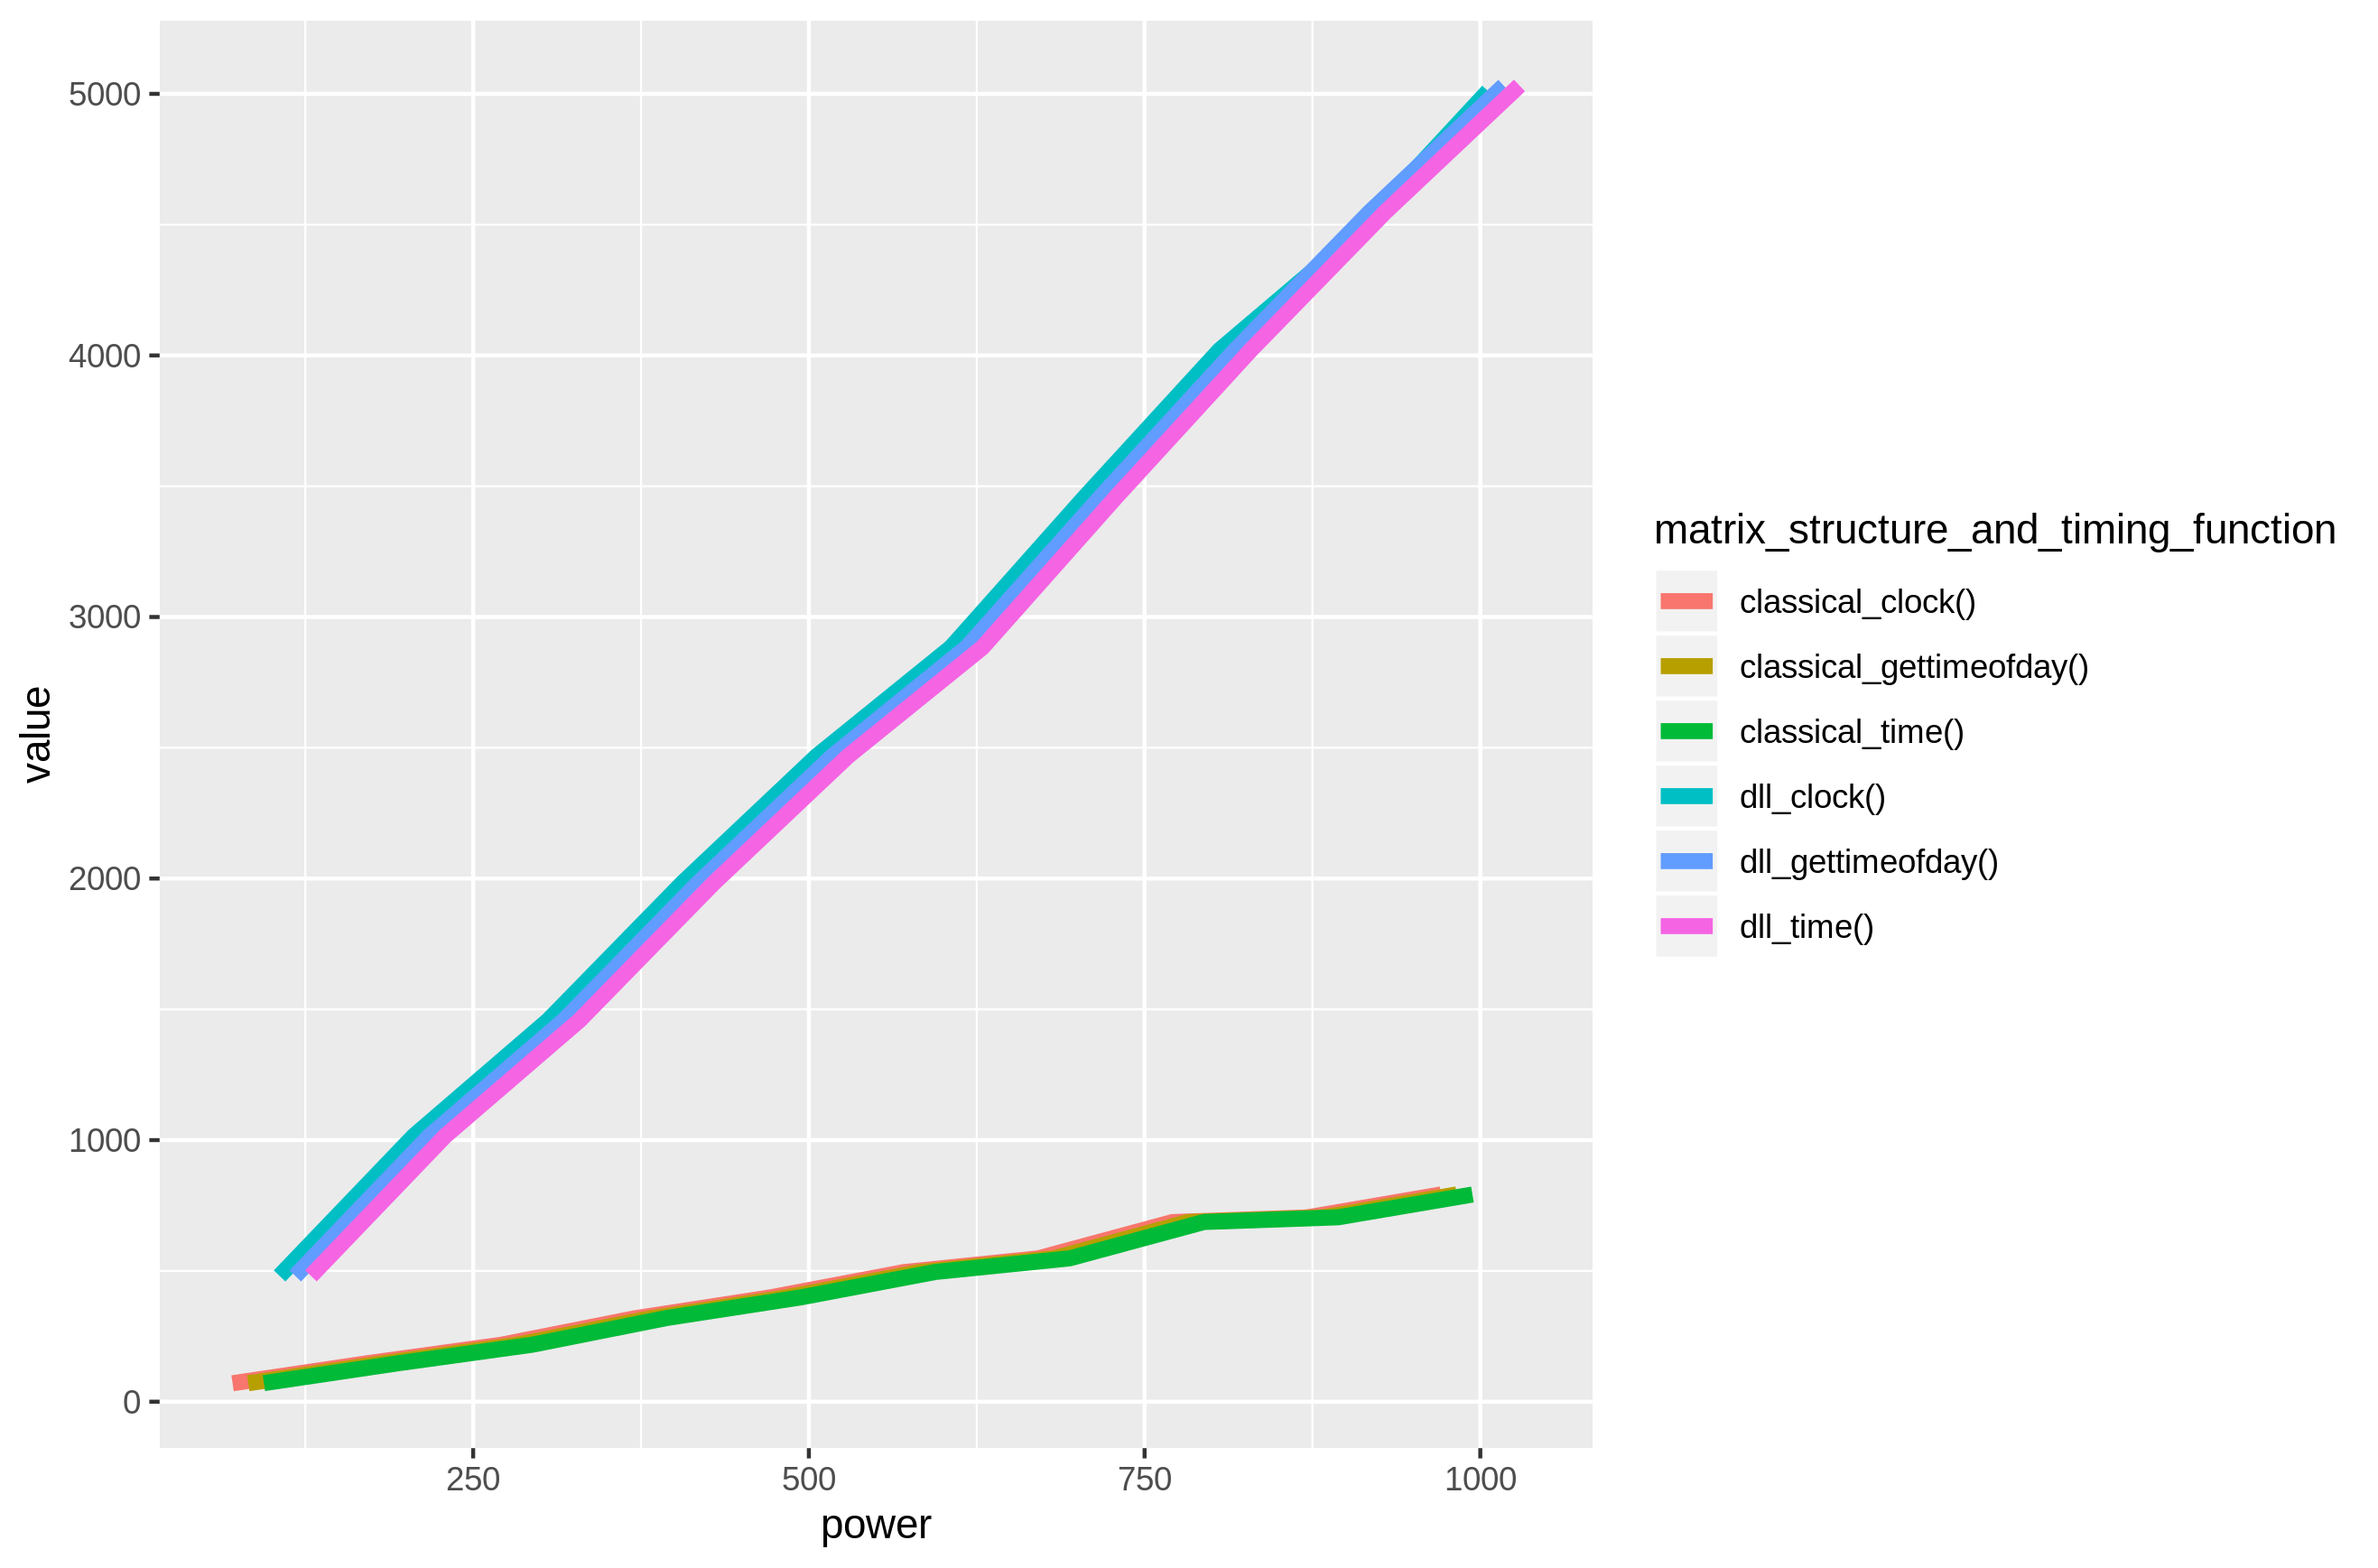
\includegraphics[width= 8cm]{../images/C_fixed_dim.png}
					\caption{C-implementation(Fixed Dimensionality and Variable Power)}
				\end{figure}
		
				
				\paragraph{Observation}
					As we can see from Figure 1 below, 
					\begin{itemize}
						\item increasing the power of the matrix increases the time complexity linearly,
						\item the classical implementation takes less time to compute the power than the double linked list implementation,
						\item time(), clock() and gettimeofday() return about the same value.
					\end{itemize}
	\newpage
				
			\subsubsection{Keeping the Power constant}
				\begin{figure}[h]
					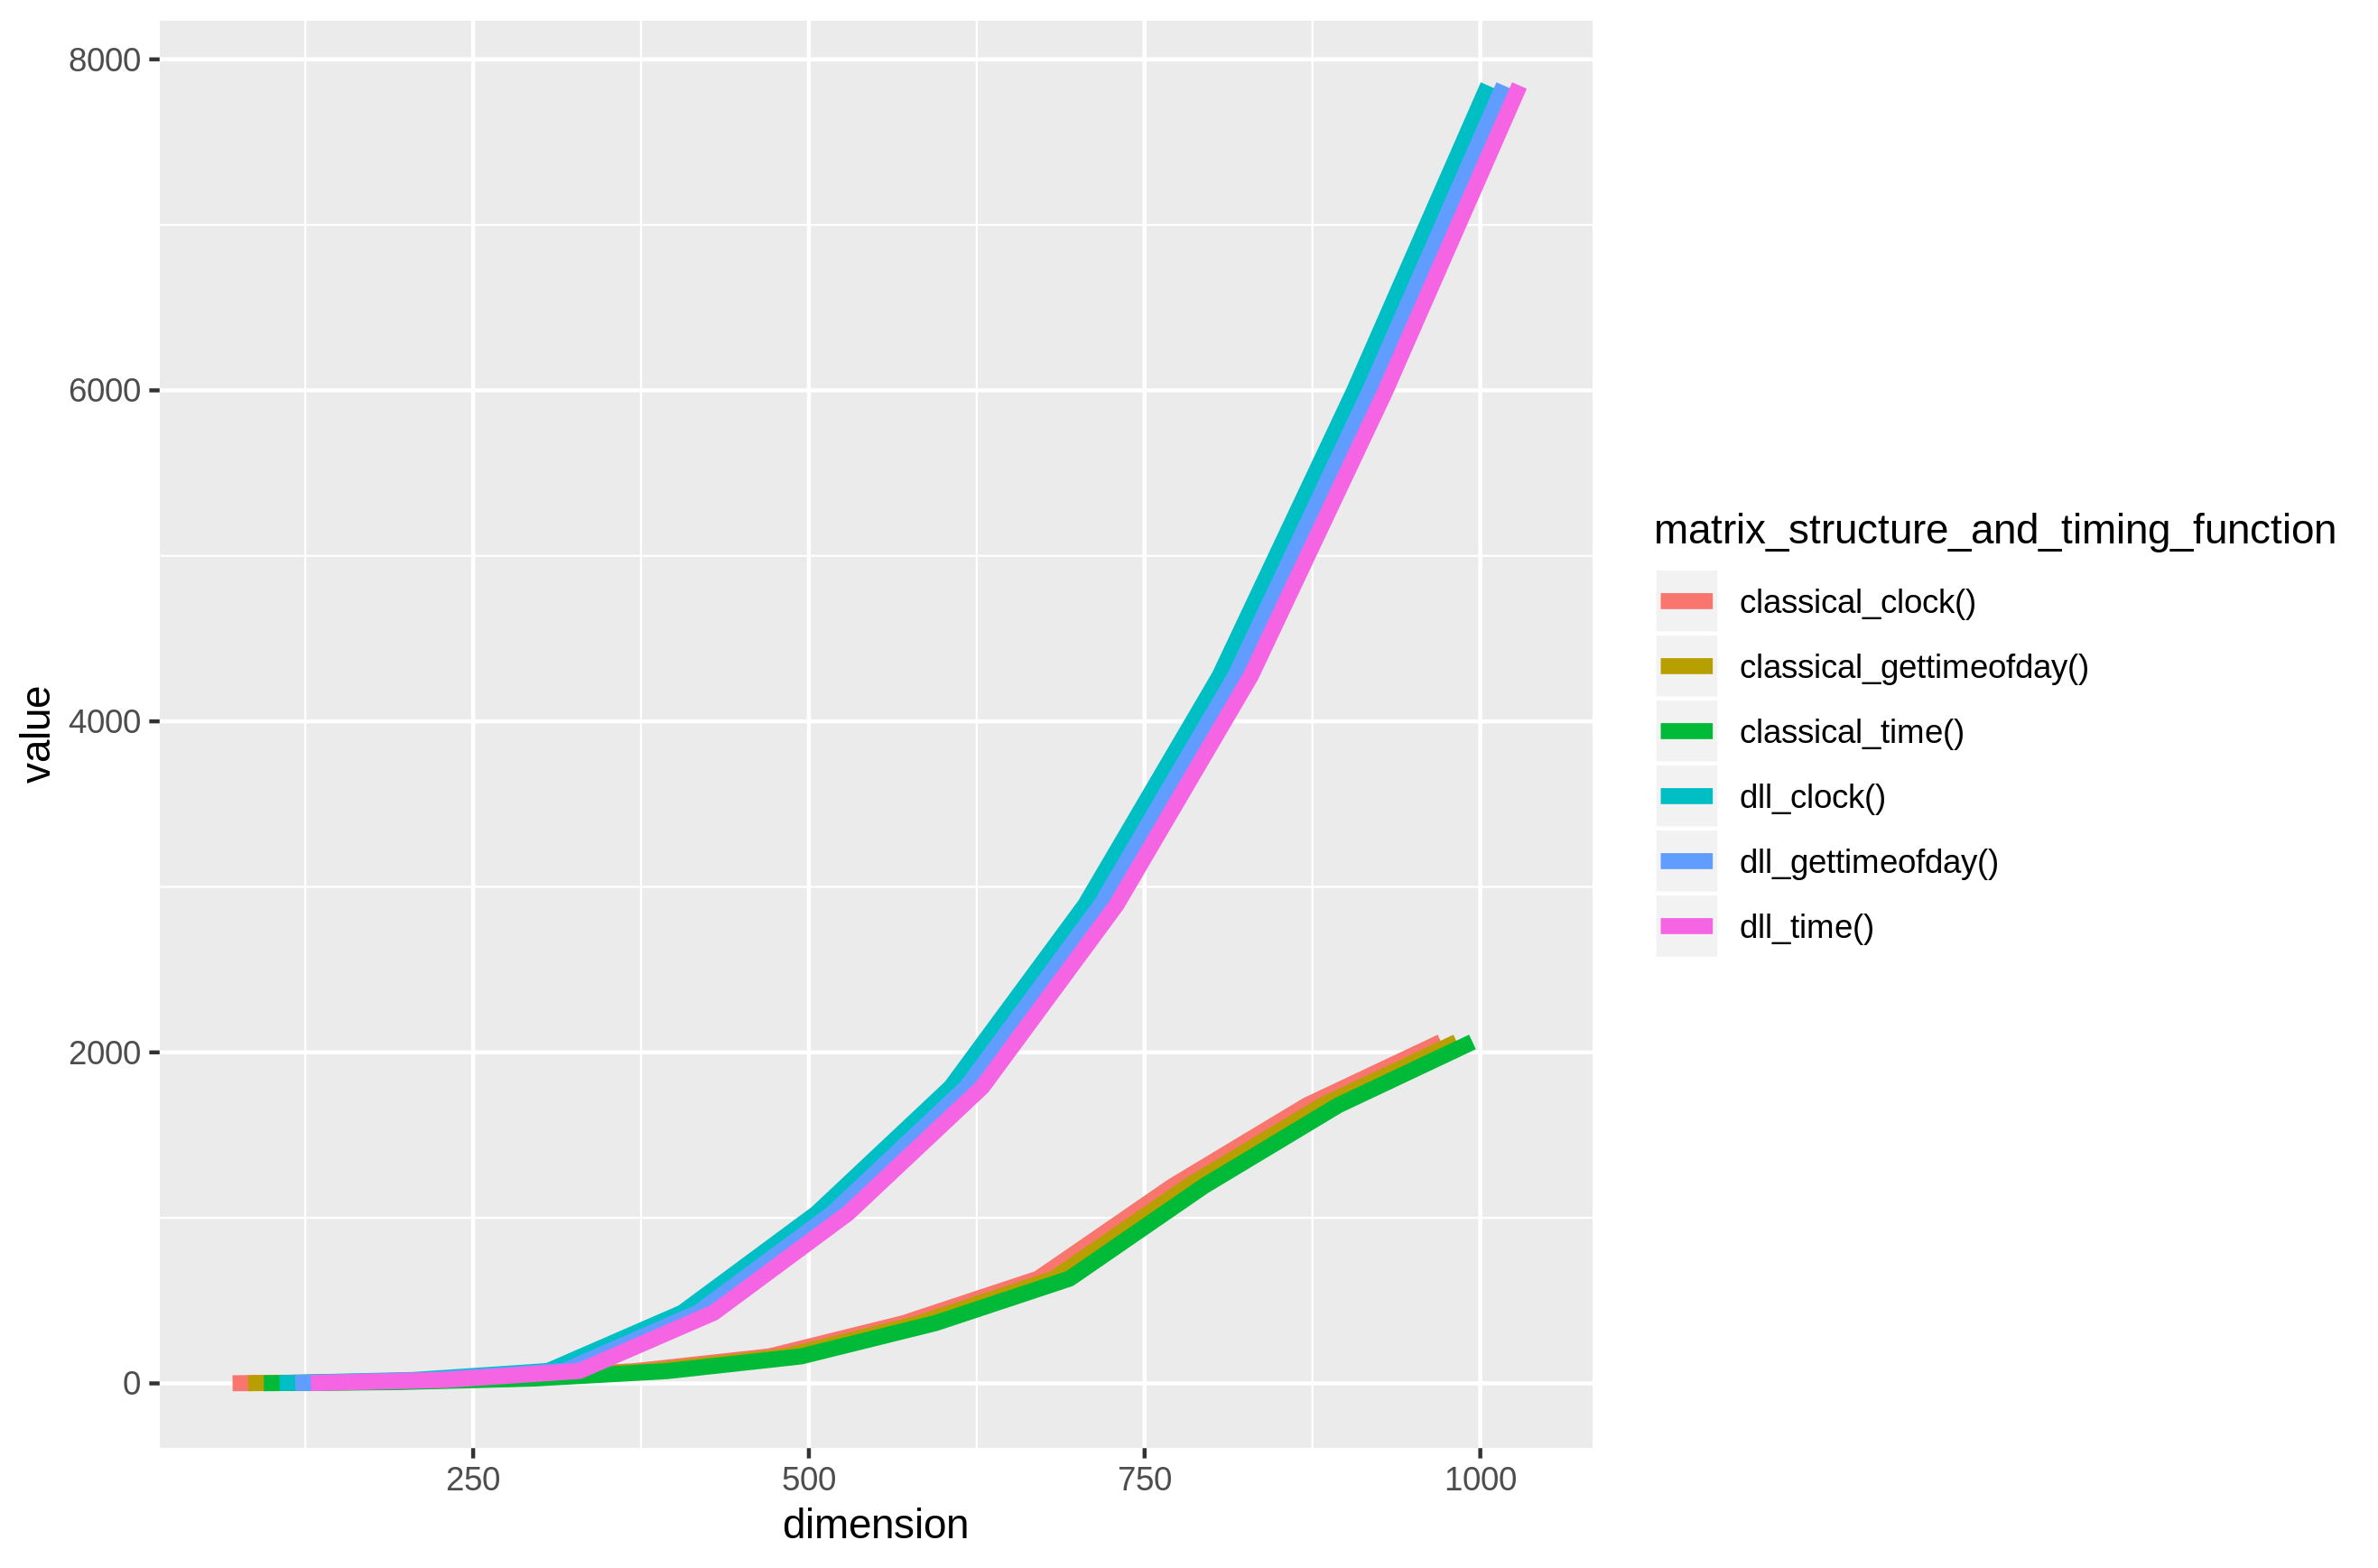
\includegraphics[width= 8cm]{../images/C_fixed_power.png}
					\caption{C-implementation(Fixed Power and Variable Dimensionality)}
				\end{figure}
				
				\paragraph{Observation}
				As we can see from Figure 2 above, 
				\begin{itemize}
					\item increasing the dimensionality of the matrix increases the time complexity exponentially,
					\item the classical implementation takes less time to compute the power than the double linked list implementation,
					\item time(), clock() and gettimeofday() return about the same value.
				\end{itemize}
		\subsection{Benchmark Using the R language}
			For the experimentation using the R language, we considered only the classical implementation of the square matrix but used two different methods to compute its power:
			\begin{itemize}
				\item using the R "\%*\%" (without the quotation marks) operator to multiply two matrices,
				\item using 3 "for loops" with the regular "*" operator to multiply two matrices.
			\end{itemize}
			Hence, the two methods above are what we are benchmarking in this section.
			
			We recorded the running times using the system.time() function which takes as input the operation or function to be timed and returns 3 different values: 
			\begin{itemize}
				\item the user CPU time: which gives the CPU time spent by the current process,
				\item the system CPU time: which gives the CPU time spent by the kernel on behalf of the current process for doing things such as opening files, looking at the system clock or starting other processes etc...,
				\item the elapsed time: which is the total elapsed time perceived by the user.
			
			\end{itemize} 
			\subsubsection{Keeping the Dimensionality constant}
				\begin{figure}[h]
					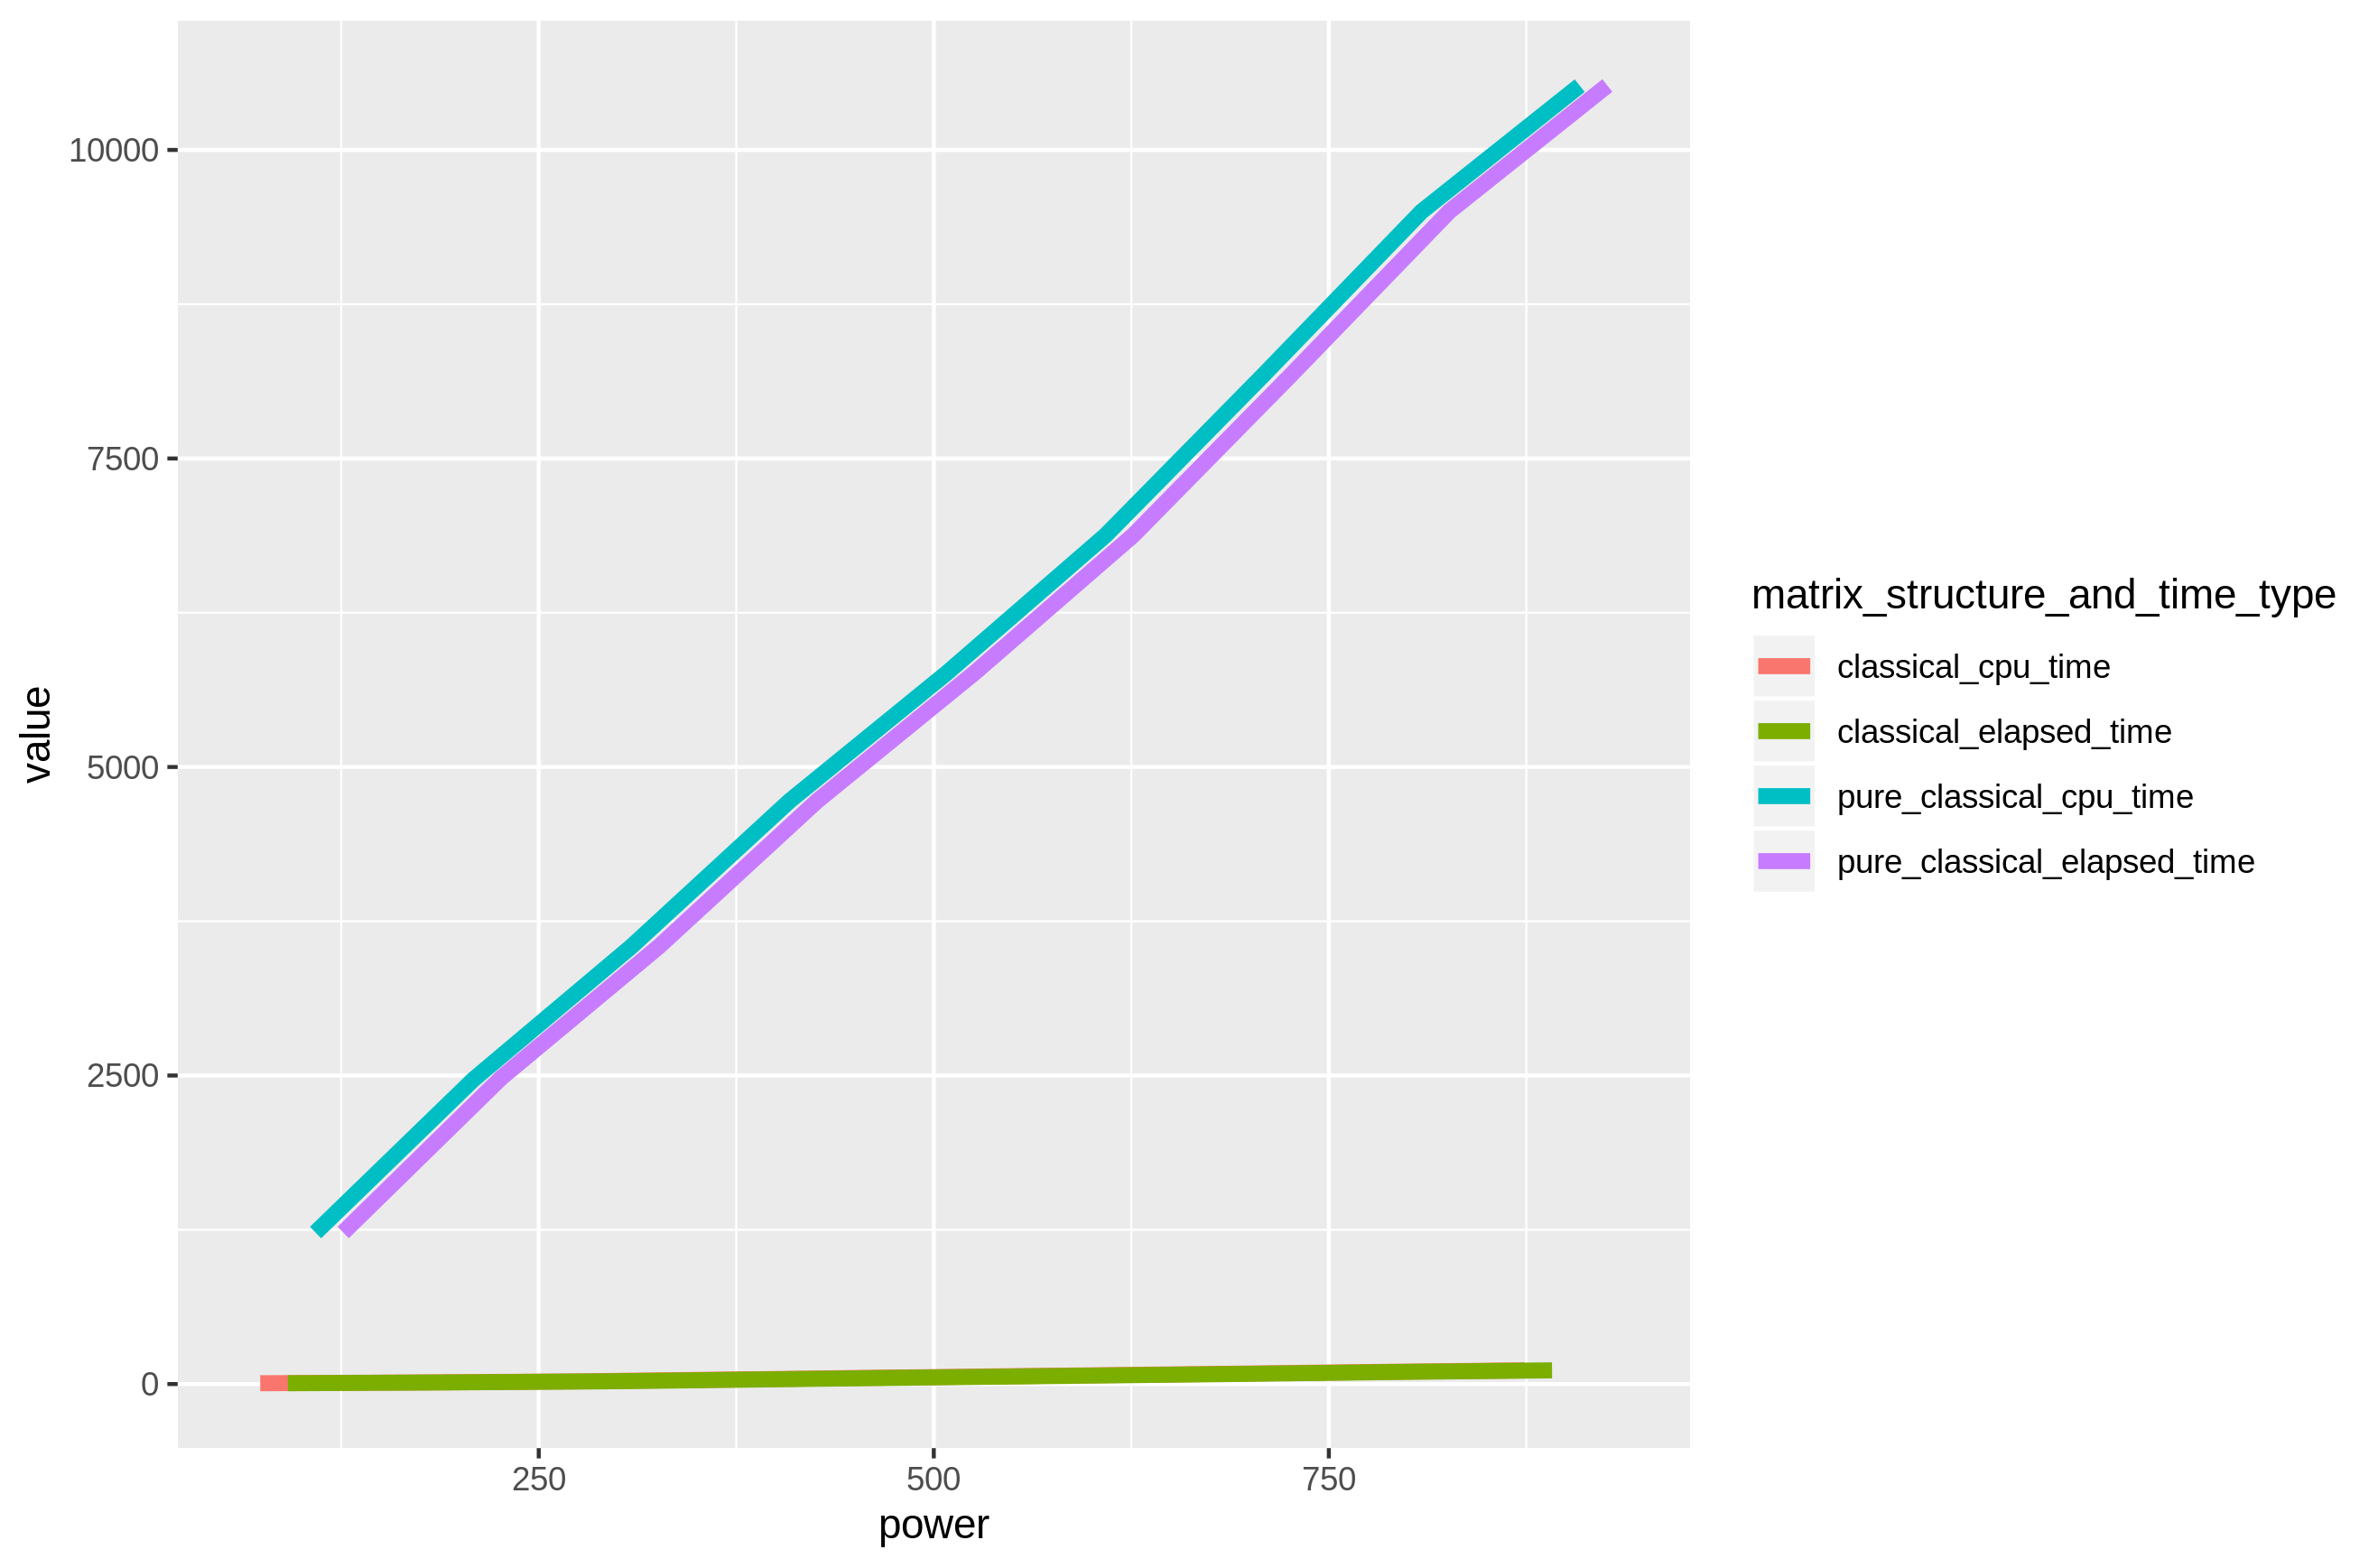
\includegraphics[width= 8cm]{../images/R_fixed_dim.png}
					\caption{R-implementation(Fixed Dimensionality and Variable Power)}
				\end{figure}
			
				\paragraph{Observation}
					As we can see from Figure 3 below, 
					\begin{itemize}
						\item increasing the power of the matrix increases the time complexity linearly,
						\item the classical implementation (i.e using the R "\%*\%" operator) takes less time to compute the power than the pure classic implementation (i.e using the "*" operator),
						\item the user CPU time is slightly better than the total elapsed time for the pure classical implementation.
					\end{itemize}
	\newpage
				
			\subsubsection{Keeping the Power constant}
				\begin{figure}[h]
					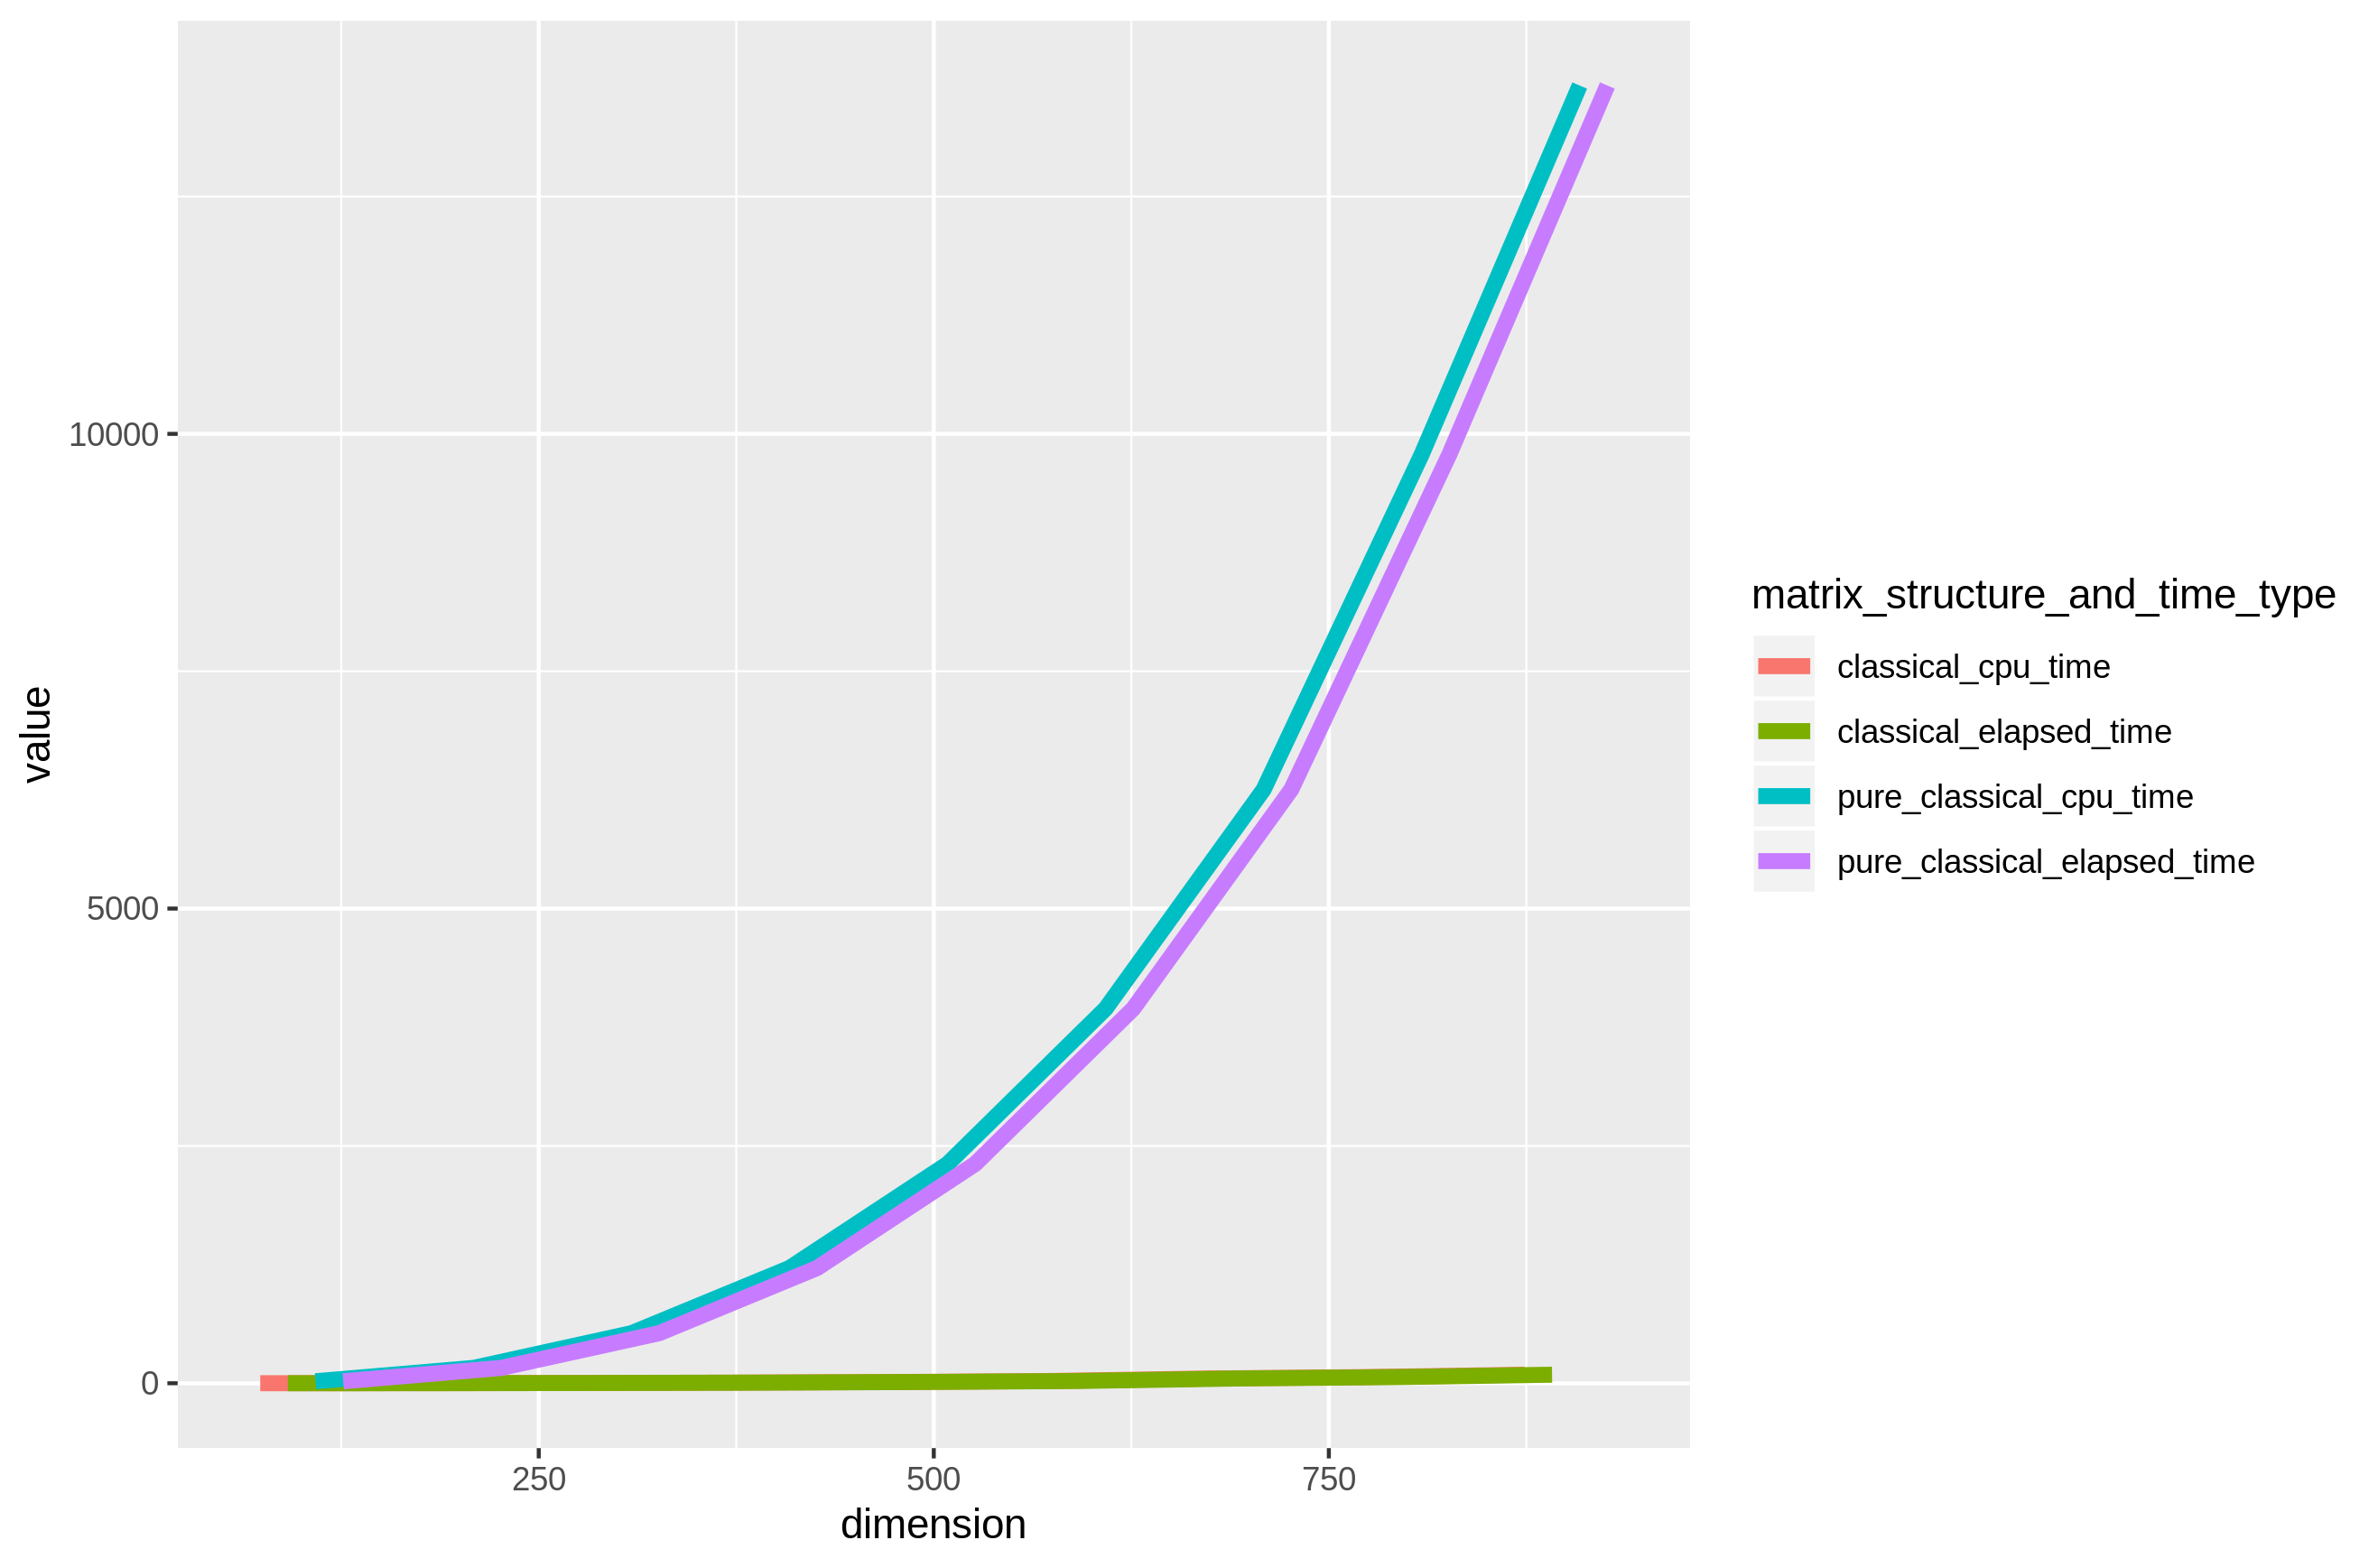
\includegraphics[width= 8cm]{../images/R_fixed_power.png}
					\caption{R-implementation(Fixed Power and Variable dimensionality)}
				\end{figure}
				
				\paragraph{Observation}
				As we can see from Figure 4 above, 
				\begin{itemize}
					\item increasing the power of the matrix increases the time complexity exponentially,
					\item the classical implementation (i.e using the R "\%*\%" operator) takes less time to compute the power than the pure classic implementation (i.e using the "*" operator),
					\item the user CPU time is slightly better than the total elapsed time for the pure classical implementation.
				\end{itemize}
		\subsection{C-classical vs R-Pure Classical}
			For this experimentation, we considered using the clock() function to record the time for the C-implementation and compared it with the "user CPU" time returned by the system.time() function on the R implementation.
			\subsubsection{Keeping the Dimensionality constant}
			\begin{figure}[h]
				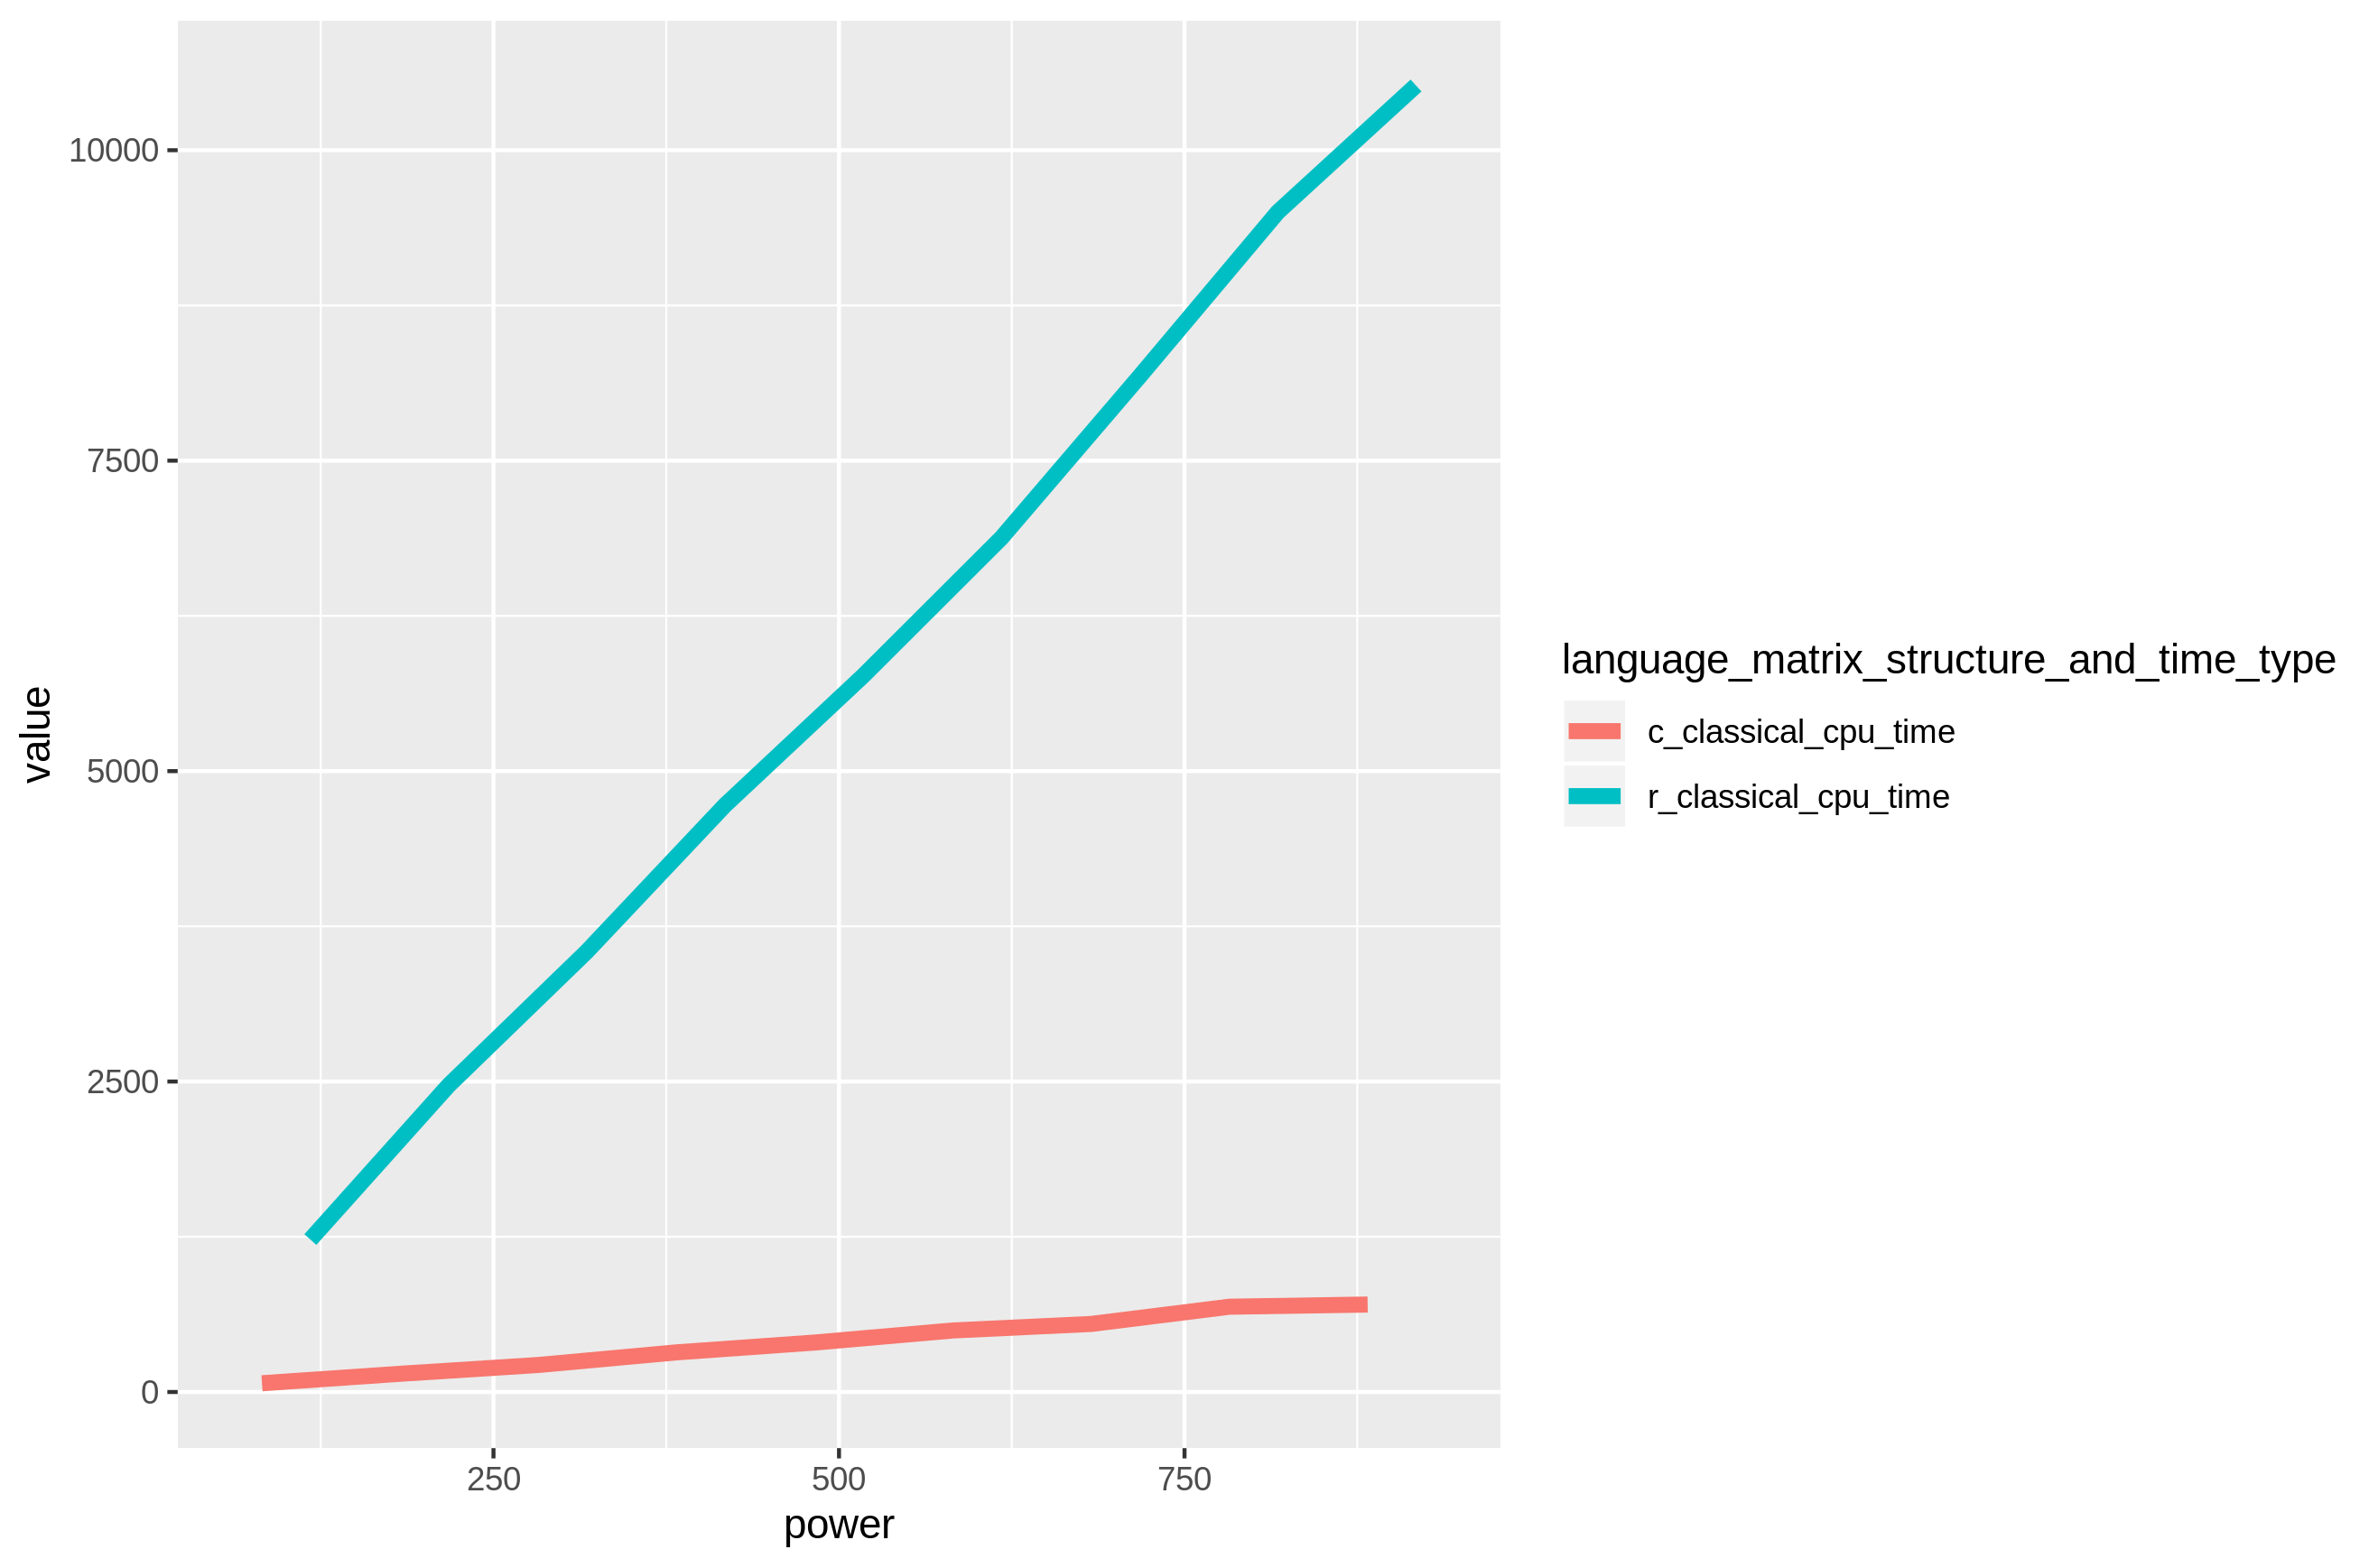
\includegraphics[width= 8cm]{../images/C_R_fixed_dim.png}
				\caption{C Vs R-implementations(Fixed Dimensionality and Variable Power)}
			\end{figure}
			
			
			\paragraph{Observation}
			As we can see from Figure 5 above, 
			\begin{itemize}
				\item increasing the power of the matrix increases the time complexity linearly,
				\item the C implementation takes less time to compute the power than the R one,
			\end{itemize}
	\newpage
		\subsubsection{Keeping the Power constant}
			\begin{figure}[h]
				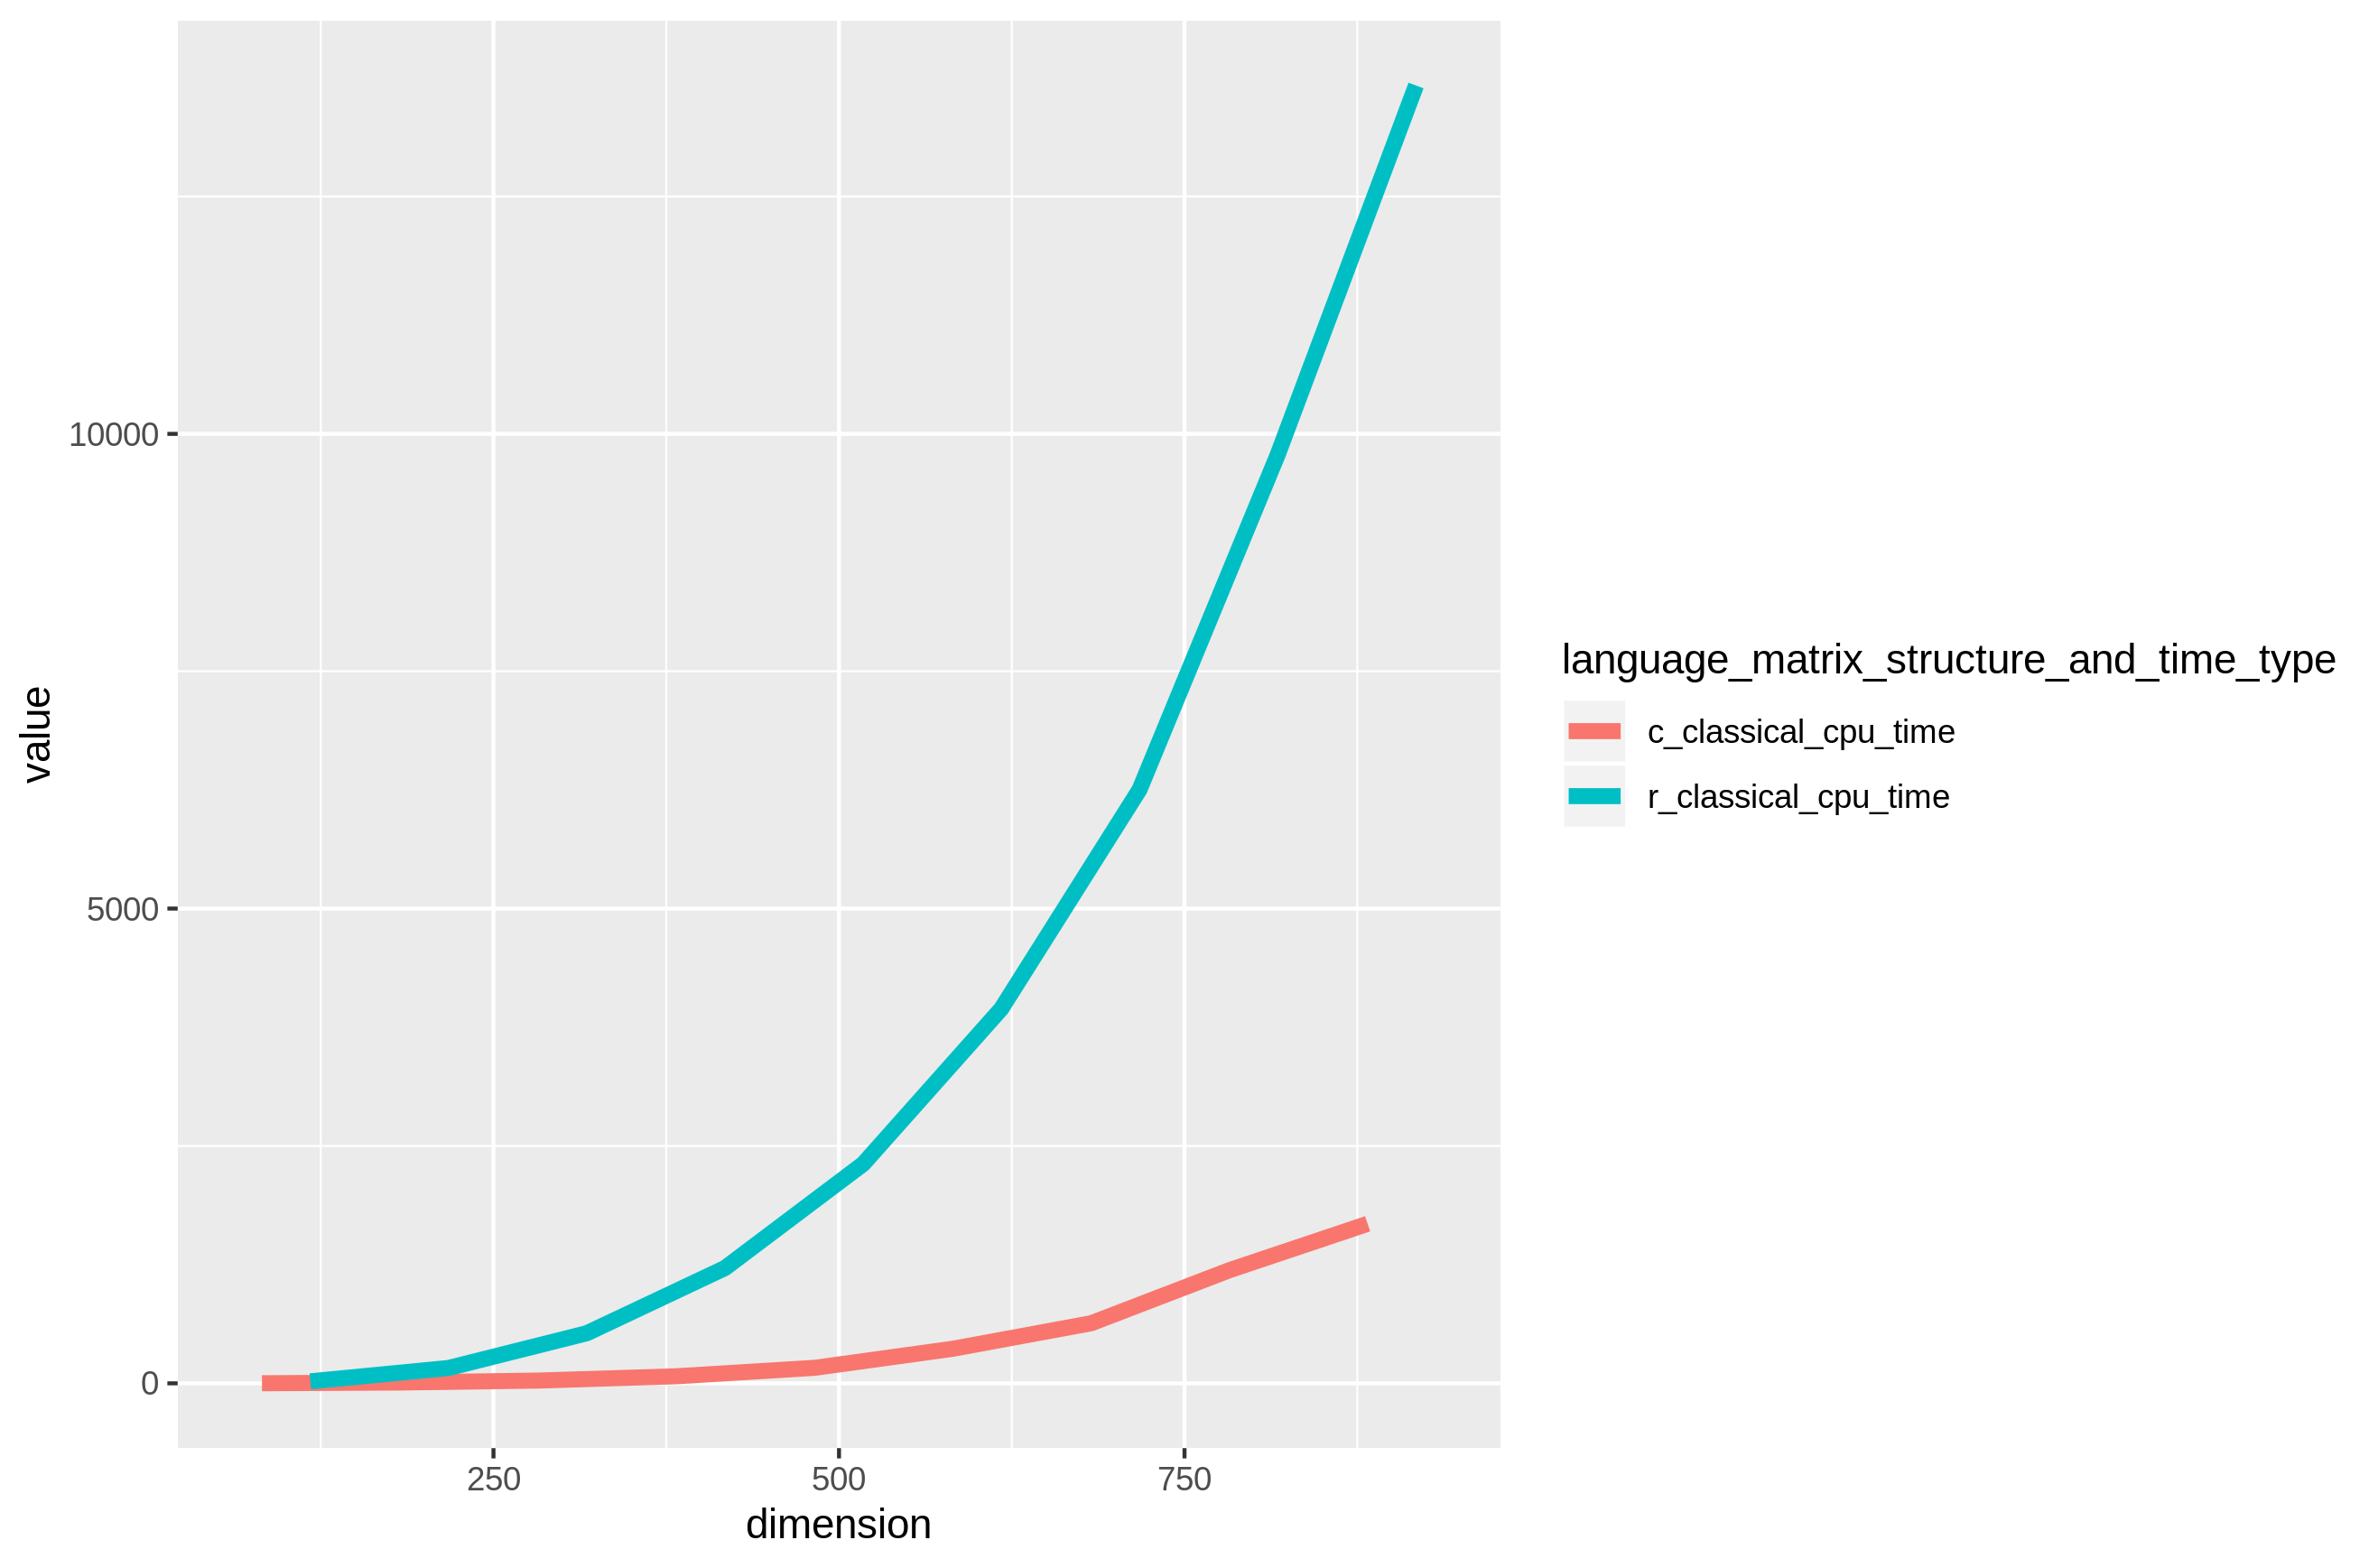
\includegraphics[width= 8cm]{../images/C_R_fixed_power.png}
				\caption{C Vs R-implementations(Fixed Power and Variable Dimensionality)}
			\end{figure}
			
			
			\paragraph{Observation}
			As we can see from Figure 6 above, 
			\begin{itemize}
				\item increasing the power of the matrix increases the time complexity exponentially,
				\item the C implementation takes less time to compute the power than the R one,
			\end{itemize}
	\section{Conclusion}
	
		After experimenting with the power of square matrices (using 2 different implementations and 2 different programming languages), we can conclude that in C, the classical implementation is faster than the double linked list one, in R, the classical implementation is faster than the pure classical one, the classical implementation in C is faster than the pure classical one in R and the classical implementation in R is better than the the classical one in C. Therefore, we recommend using the R classical implementation to compute the power of a large matrix.	
\end{document}